% generated by Docutils <http://docutils.sourceforge.net/>
\documentclass[letterpaper,landscape,english,9pt]{report}
\usepackage[landscape,margin=0.5cm]{geometry}

\usepackage{fixltx2e} % LaTeX patches, \textsubscript
\usepackage{cmap} % fix search and cut-and-paste in PDF
\usepackage[T1]{fontenc}
\usepackage[utf8]{inputenc}
\usepackage{ifthen}
\usepackage{babel}
\usepackage{color}
\usepackage{float} % float configuration
\floatplacement{figure}{H} % place figures here definitely


\usepackage{multicol}
%\setlength{\columnseprule}{1pt} % for visible divider
\setlength{\columnsep}{1cm}

\usepackage{graphicx}
\graphicspath{
 {../pics/}
}

%%% Custom LaTeX preamble
% PDF Standard Fonts
\usepackage{mathptmx} % Times
\usepackage[scaled=.90]{helvet}
\usepackage{courier}

\usepackage{flowfram}
%\usepackage{booktabs}           % for rules in tables
\usepackage{tabularx}           % for column-width tables
\usepackage[table]{xcolor}      % color control

%\usepackage[colorlinks]{hyperref}

\usepackage{enumitem}           % useful for control of listings
\usepackage[compact,raggedright]{titlesec}
\usepackage{comment}

\newcommand{\epigraph}[3]{\textit{#1}\linebreak \vspace{-1.5em} \begin{flushright}\hspace{5em}\ --\ #2\linebreak\small{#3} \end{flushright}}

\pagestyle{empty}
\parindent=0pt

% Attempts to change bg color of *section headings
%\definecolor{secbgcol}{rgb}{0.9, 0.85, 0.85}
%\titleformat{\section}
%{\color{red}\normalfont\Large\bfseries}{\ndsection}{1em}{}
%\titleformat{\subsection}
%{\color{red}\normalfont\large\bfseries}{\begin{flushright}\hfill\thesubsection
%  \end{flushright}}{1em}{}
%
%\usepackage{pstricks}

% To create tables within multicols
\makeatletter
\newenvironment{ndtable}
  {\def\@captype{table}}
  {}


\newcommand{\ndheading}[3]{%
\vspace{0.5em}
\begin{ndtable}%
\rowcolors[\hline]{1}{#2}{} \arrayrulecolor{#3}
\begin{tabularx}{\columnwidth}{>{\centering\arraybackslash}X}\vspace{-.5em}\normalfont\large\bfseries
  #1\vspace{0.05em}\\\end{tabularx}
\end{ndtable}
\vspace{-.5em}
}

\definecolor{secfgcol}{RGB}{102, 153, 0}
\definecolor{secbgcol}{RGB}{216, 255, 137}
\definecolor{projfgcol}{RGB}{6,   83, 215}
\definecolor{projbgcol}{RGB}{255, 255, 205}

%\definecolor{secfgcol}{RGB}{6, 83, 215}
%\definecolor{secbgcol}{RGB}{241, 248, 255}
%\definecolor{projfgcol}{RGB}{6,   83, 215}
%\definecolor{projbgcol}{RGB}{241, 248, 255}

\newcommand{\ndsection}[1]{\ndheading{#1}{secbgcol}{secfgcol}}
\newcommand{\ndsubsection}[1]{\ndheading{#1}{secbgcol}{secfgcol}}

%\newcommand{\ndproject}[2]{\ndheading{\noindent#1\newline{\small\url{#2}}}{secbgcol}{secfgcol}}

\newcolumntype{V}{>{\arraybackslash} m{.2\linewidth} }
\newcolumntype{C}{>{\arraybackslash} m{.7\linewidth} }
\newcommand{\ndproject}[6]{%
\vspace{0.5em}
\begin{ndtable}%
\rowcolors[]{1}{projbgcol}{} \arrayrulecolor{projbgcol}
\begin{tabularx}{\columnwidth}{CV}\vspace{-.5em}\normalfont\large\bfseries
 #1 \newline {\small\url{#2}} &
 \vspace{#5}\hspace{#6}\includegraphics[width=#4\columnwidth]{../pics/#3}\vspace{-0.5em}\end{tabularx}
\end{ndtable}
\vspace{-.5em}
}

\newcommand{\ndcite}[1]{{\small #1}}
%%% User specified packages and stylesheets

%%% Fallback definitions for Docutils-specific commands

% admonition (specially marked topic)
\providecommand{\DUadmonition}[2][class-arg]{%
  % try \DUadmonition#1{#2}:
  \ifcsname DUadmonition#1\endcsname%
    \csname DUadmonition#1\endcsname{#2}%
  \else
    \begin{center}
      \fbox{\parbox{0.9\textwidth}{#2}}
    \end{center}
  \fi
}

% title for topics, admonitions and sidebar
\providecommand*{\DUtitle}[2][class-arg]{%
  % call \DUtitle#1{#2} if it exists:
  \ifcsname DUtitle#1\endcsname%
    \csname DUtitle#1\endcsname{#2}%
  \else
    \smallskip\noindent\textbf{#2}\smallskip%
  \fi
}

% hyperlinks:
\ifthenelse{\isundefined{\hypersetup}}{
  \usepackage[unicode,colorlinks=true,linkcolor=blue,urlcolor=blue]{hyperref}
  \urlstyle{same} % normal text font (alternatives: tt, rm, sf)
}{}
\hypersetup{
  pdftitle={Python in NeuroImaging},
}

%%% Body
\begin{document}

\begin{multicols}{3}    % 3 columns

% Document title
%\section*{
\begin{center}\Large \textbf{Python in NeuroImaging}\end{center}
%}
%\label{python-in-neuroimaging}

\begin{center}
\noindent
\includegraphics[width=0.5\columnwidth]{snakebrain}
%\includegraphics[width=0.5\columnwidth]{openlogo-vsop}

Find the community @ \url{http://www.nipy.org}
%\ndsection{Debian GNU/Linux}

% \hrule
\end{center}
\vspace{0em}

%___________________________________________________________________________

\ndsection{Stimuli Delivery}

%___________________________________________________________________________

\ndproject{PsychoPy}{http://www.psychopy.org}{psychopy_logo.pdf}{.2}{-0.25em}{0em}

%\begin{figure}
%
\includegraphics[width=0.3\columnwidth]{../pics/psychopy_logo.pdf}
%\end{figure}

PsychoPy is an easy, precise, platform-independent package for
stimulus presentation. Suitable for psychophysics, neuroimaging, and
all areas of psychology.
\begin{itemize}[nolistsep,topsep=0em,leftmargin=1pc]
\item Huge variety of stimuli generated in real-time
\item Cross-platform -- run the same script on Linux, Win or OS X
\item Flexible stimulus units (degrees, cm, or pixels)
\item Coder interface for those that like to program
\item Builder interface for those that don’t
\item Input from keyboard, mouse, joystick or button boxes
\item Multi-monitor support
\item Automated monitor calibration (supported photometers)
\end{itemize}
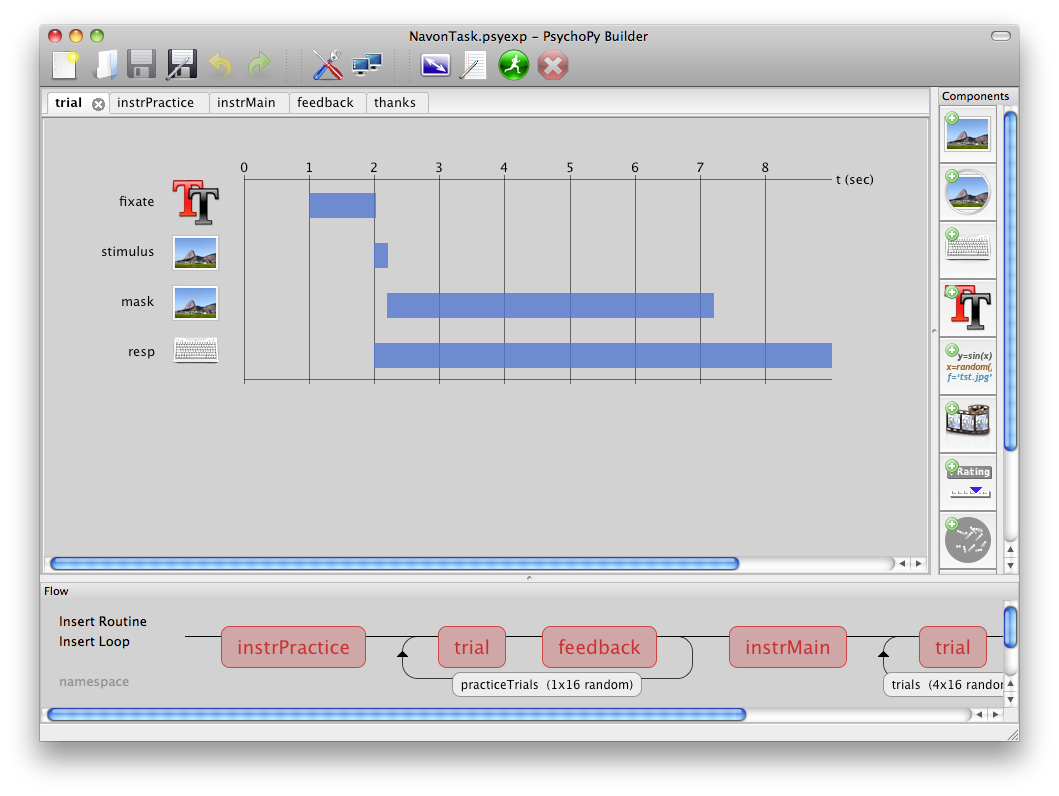
\includegraphics[width=\columnwidth]{../pics/psychopyBuilder.png}
\vspace{-2em}

%___________________________________________________________________________

\ndproject{OpenSesame}{http://www.cogsci.nl/software/opensesame}{opensesame_logo.pdf}{.2}{-0.25em}{0em}

OpenSesame is a graphical experiment builder for the social sciences.
\begin{itemize}[nolistsep,topsep=0em,leftmargin=1pc]
\item A comprehensive and intuitive graphical user interface
\item WYSIWYG drawing tools for creating visual stimuli
\item Cross-platform % compatibility (Windows, Linux, Mac OS)
\item Python scripting for complex tasks
\item A plug-in framework
\item Compatibility (through plug-ins) with commonly used devices:
  (e.g. Eyelink eye trackers, serial response boxes, Mantra object tracker)
\item Compatibility with popular Python libraries:
  PsychoPy, PyGame, PyOpenGL, etc.
\end{itemize}
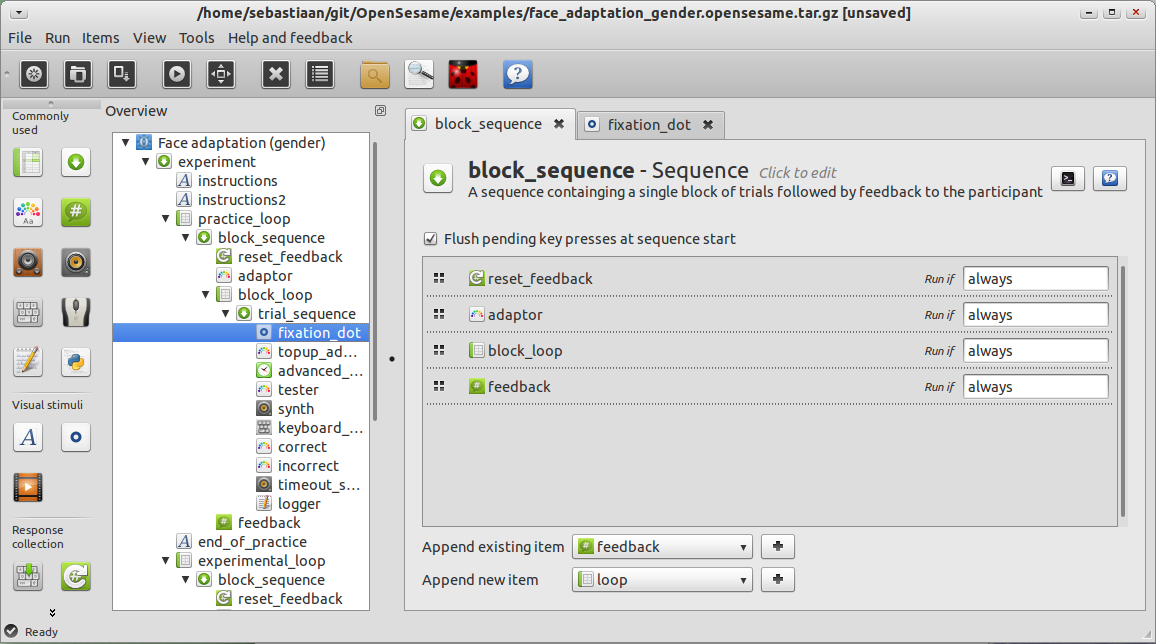
\includegraphics[width=\columnwidth]{../pics/opensesame_screenshot2.png}


%___________________________________________________________________________
\ndsection{Data I/O}

\ndproject{NiBabel}{http://nipy.org/nibabel}{reggie.png}{.2}{-4.25em}{0em}

Nibabel provides read and write access to some common medical and
neuroimaging file formats, including:
\href{http://www.grahamwideman.com/gw/brain/analyze/formatdoc.htm}{ANALYZE}
(plain, SPM99, SPM2),
\href{http://www.nitrc.org/projects/gifti}{GIFTI},
\href{http://nifti.nimh.nih.gov/nifti-1/}{NIfTI1},
\href{http://wiki.bic.mni.mcgill.ca/index.php/MINC}{MINC}, as well as
PAR/REC. NiBabel is the successor of
\href{http://niftilib.sourceforge.net/pynifti/}{PyNIfTI}.

The various image format classes give full or selective access to
header (meta) information and access to the image data is made
available via NumPy arrays.


%___________________________________________________________________________

\ndsection{Analysis}%

%___________________________________________________________________________

\ndproject{BrainVISA}{http://brainvisa.info}{brainvisa_logo.png}{.2}{-0.25em}{0em}

BrainVISA is an open-source, modular and customizable software platform built
to host heterogeneous tools dedicated to neuroimaging research. It aims at
helping researchers in developing new neuroimaging tools, sharing data and
distributing their software.
\begin{itemize}[nolistsep,topsep=0em,leftmargin=1pc]
%\item Written in pure Python
\item Databasing capabilities
\item Massive computation facilities using Soma-workflow
\item Open environment, with many toolboxes
\item Specialized toolboxes for T1 MRI processing, sulci ang gyri morphometry,
diffusion imaging and fibers tracking, surfacic and structural analysis,
3D histology\ldots
\item Links with other software like SPM, FSL, FreeSurfer, or CIVET
\end{itemize}
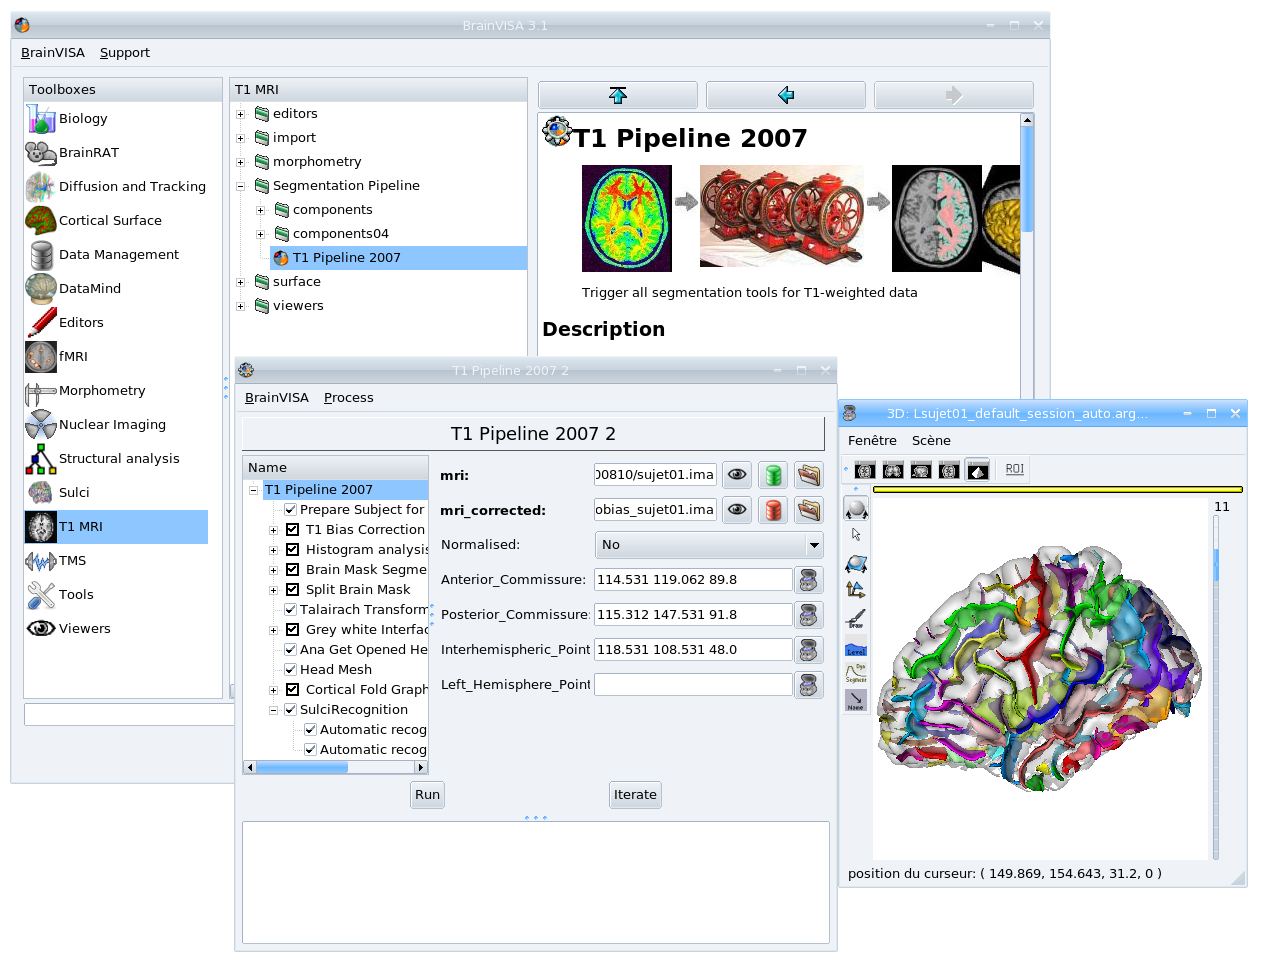
\includegraphics[width=\columnwidth]{../pics/brainvisa_screenshot.png}
\ndcite{D. Geffroy, D. Rivière, I. Denghien, N. Souedet,
  S. Laguitton, and Y. Cointepas. BrainVISA: a complete software
  platform for neuroimaging.  In Python in Neuroscience workshop,
  Paris, Aug. 2011.}

%___________________________________________________________________________

\ndproject{DiPy}{http://nipy.org/dipy}{dipy-banner.png}{.5}{-0.25em}{-7.2em}

Dipy is an international FOSS project for diffusion magnetic resonance
imaging analysis.  Dipy is multiplatform and will run under any
standard operating system such as \emph{Windows}, \emph{Linux},
\emph{Mac OS X}.  Some of our \textbf{state-of-the-art} applications
are:
\begin{itemize}[nolistsep,topsep=0em,leftmargin=1pc]
\item Reconstruction algorithms e.g. GQI, DTI
\item Tractography generation algorithms e.g. EuDX
\item Intelligent downsampling of tracks
\item Ultra fast tractography clustering
\item Resampling datasets with anisotropic voxels to isotropic
\item Visualizing multiple brains simultaneously
\item Finding track correspondence between different brains
\item Warping tractographies into another (e.g. MNI) space
\item Support of various  file formats e.g. Trackvis or NIfTI
%\item Dealing with huge tractographies without memory restrictions
%\item Playing with datasets interactively without storing
\end{itemize}

%___________________________________________________________________________

\ndproject{NiPy}{http://nipy.org/nipy}{blank.png}{.2}{-1.25em}{0em}

NIPY provides a rich suite of algorithms for pre-processing and
analysis of neuroimaging data
\begin{itemize}[nolistsep,topsep=0em,leftmargin=1pc]
\item General linear model (GLM) statistical analysis
\item Combined slice time correction and motion correction
\item General image registration routines with flexible cost functions, optimizers
and resampling schemes
\item Image segmentation
\item Basic visualization of results in 2D and 3D
\item Basic time series diagnostics
\item Clustering and activation pattern analysis across subjects
\item Reproducibility analysis for group studies
\end{itemize}
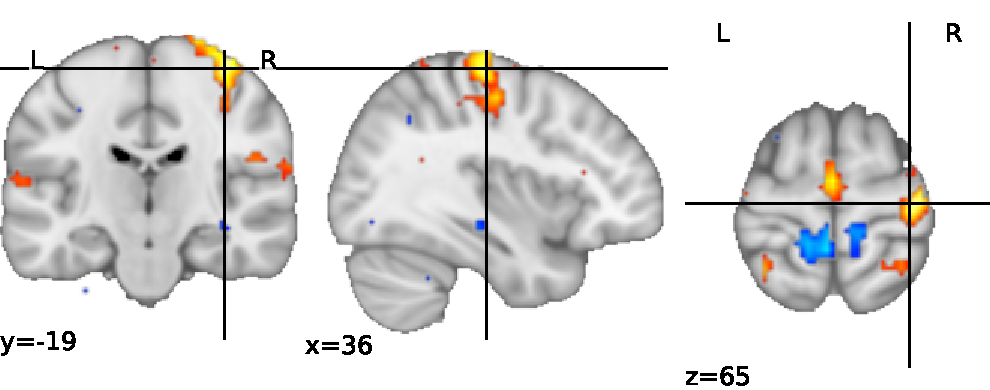
\includegraphics[width=\columnwidth]{../pics/nipy_viz.pdf}

%___________________________________________________________________________

\ndproject{Nipype}{http://nipy.org/nipype}{blank.png}{.2}{-1.25em}{0em}

Nipype provides an environment that encourages interactive exploration
of algorithms from different packages (e.g., SPM, FSL, FreeSurfer,
Camino, AFNI, Slicer), eases the design of workflows within and
between packages, and reduces the learning curve necessary to use
different packages.
% Nipype is creating a collaborative platform for
%neuroimaging software development in a high-level language and
%addressing limitations of existing pipeline systems. 
Nipype allows you to
\begin{itemize}[nolistsep,topsep=0em,leftmargin=1pc]
\item interact with tools from different software packages
\item combine processing steps from different packages
\item develop new workflows faster by reusing common steps from old ones
\item process data faster by running in parallel% on many cores/machines
\item make your research easily reproducible
\item share your processing workflows with the community
\end{itemize}
\vspace{-1em}
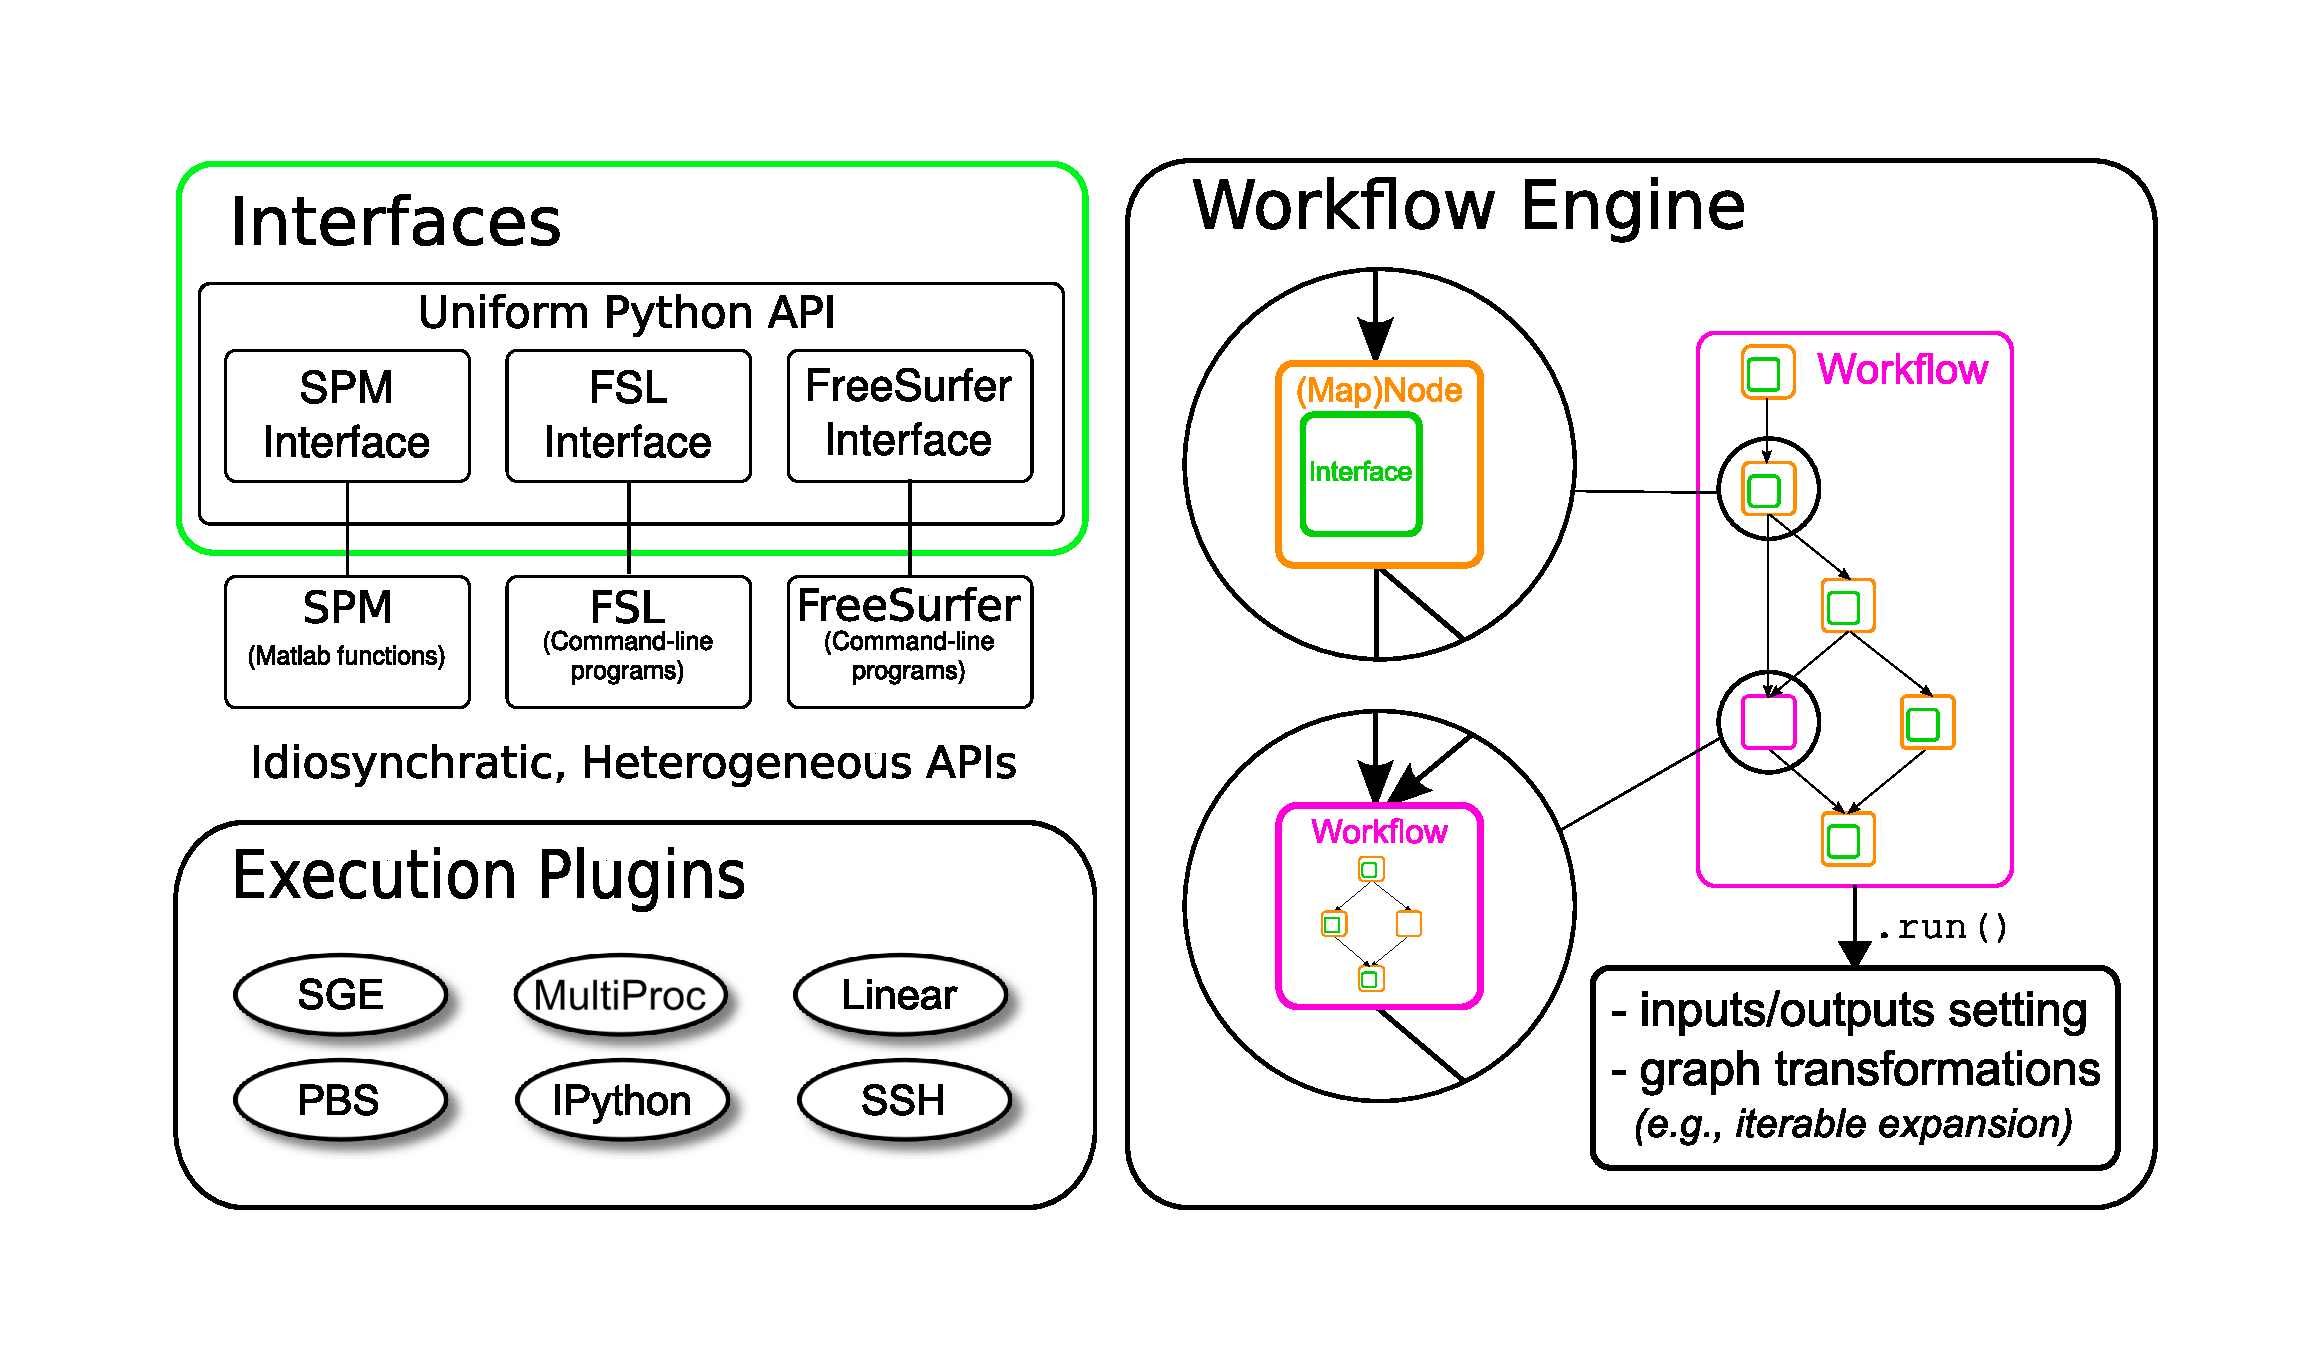
\includegraphics[width=\columnwidth]{nipype_arch.pdf}
%\vspace{-3em}

\ndcite{Gorgolewski K, Burns CD, Madison C, Clark D,
  Halchenko YO, Waskom ML, Ghosh SS (2011) Nipype: a flexible,
  lightweight and extensible neuroimaging data processing framework in
  Python. Front. Neuroinform. 5:13.  doi: 10.3389/fninf.2011.00013}


%___________________________________________________________________________

\ndproject{NiTime}{http://nipy.org/nitime}{nitime_logo.pdf}{.3}{-1.25em}{-3em}

Nitime is a library for time-series analysis of data from neuroscience
experiments.  It contains a core of numerical algorithms for
time-series analysis both in the time and spectral domains, a set of
container objects to represent time-series, and auxiliary objects that
expose a high level interface to the numerical machinery and make
common analysis tasks easy to express with compact and semantically
clear code.
\begin{itemize}[nolistsep,topsep=0em,leftmargin=1pc]
\item Spectral transforms (e.g. multi-tapered spectral analysis) and
filtering
\item Connectivity measures (Correlation, Coherency, Granger 'causality')
\item Event-related analysis (e.g. OLS FIR).
\end{itemize}
%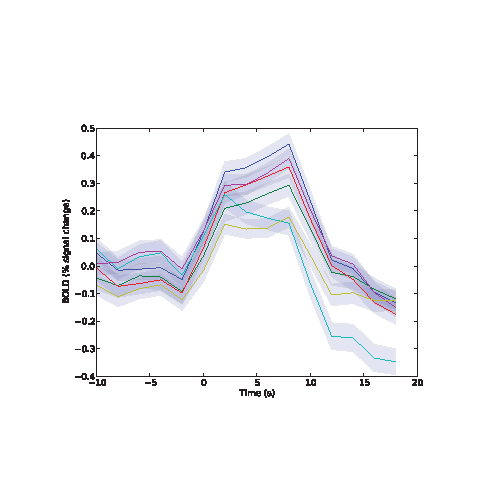
\includegraphics[width=\columnwidth]{nitime_analysis.pdf}
%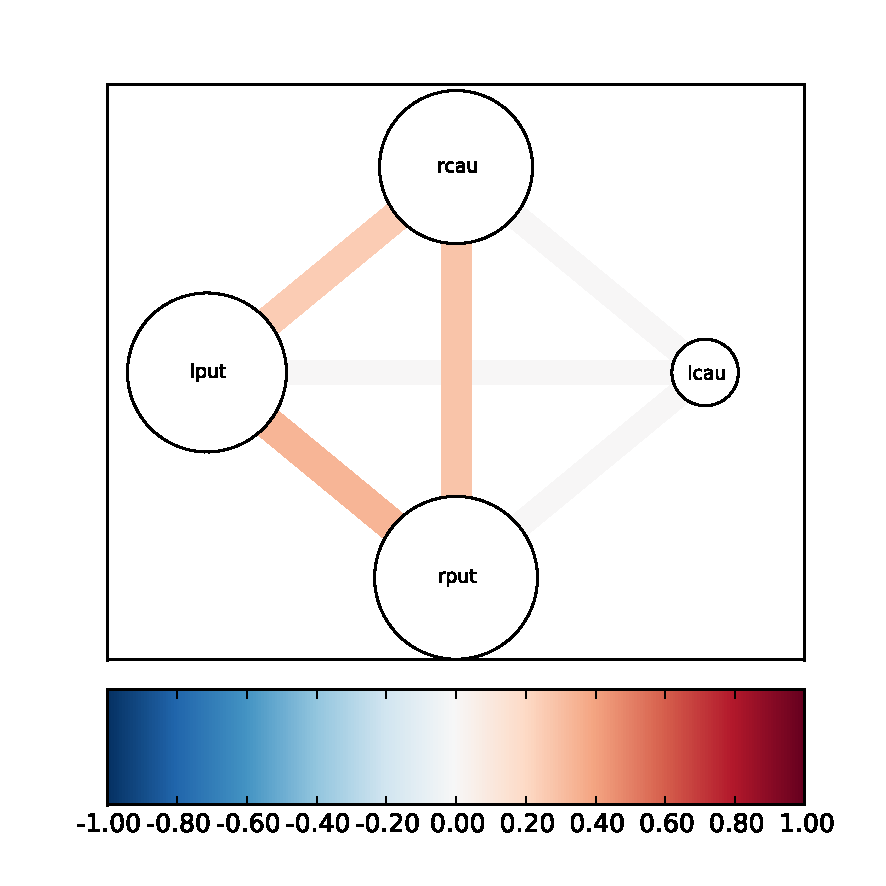
\includegraphics[width=0.9\columnwidth]{nitime_network.pdf}

%___________________________________________________________________________

\ndproject{PyMVPA}{http://www.pymvpa.org}{pymvpa_logo.pdf}{.45}{-0.25em}{-6em}

PyMVPA eases statistical learning analyses (or otherwise called
Multivariate pattern analysis, MVPA) of large datasets, with an accent
on neuroimaging.
\begin{itemize}[nolistsep,topsep=0em,leftmargin=1pc]
\item Easy I/O to Neuroimaging data (via NiBabel)
\item Variety of machine learning methods (e.g. SVM, SMLR, kNN)
\item Uniform interfaces to other toolkits (e.g. MDP, Shogun, Scikit-learn)
\item Flexible Searchlight-ing
\item Uber-Fast GNB Searchlight-ing
\item Hyperalignment (Haxby et al 2011, Neuron)
\end{itemize}
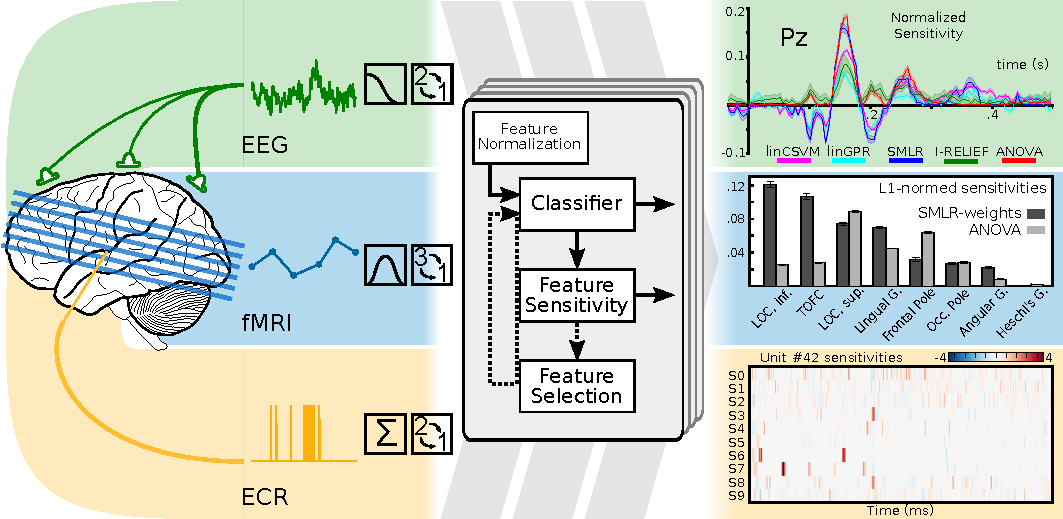
\includegraphics[width=\columnwidth]{pymvpa_shot.pdf}
\ndcite{Hanke, M., Halchenko, Y. O., Sederberg, P. B., Hanson,
  S. J., Haxby, J. V.  \& Pollmann, S. (2009).
  PyMVPA: A Python toolbox for multivariate pattern analysis of fMRI data. Neuroinformatics}\\
%\ndcite{Haxby, J. V. , Guntupalli, J. S. , Connolly, A. C. ,
%  Halchenko, Y. O. , Conroy, B. R., Gobbini, M. I. , Hanke, M. and
%  Ramadge, P. J. (2011). A Common, High-Dimensional Model of the
%  Representational Space in Human Ventral Temporal Cortex. Neuron,
%  72.}

%___________________________________________________________________________

% \ndproject{AIMS}{http://brainvisa.info}{blank.png}{.2}{-2.25em}{0em}
% 
% AIMS is the image processing library provided within the BrainVISA environment.
% It is independent from BrainVISA, and the basis for the Anatomist viewer.
% \begin{itemize}[nolistsep,topsep=0em,leftmargin=1pc]
% \item C++ and Python APIs, including integration with Numpy arrays
% \item Open and plugin-based IO system supporting various volume formats (NIFTI-1,
% Analyze, DICOM, MINC, ECAT, and several others including all standard 2D
% image formats), several mesh and texture formats (GIFTI, PLY,
% % CIVET, BrainVisa Mesh and Tri, export as VRML-1, POV, 
% \ldots), graphs.
% \item Many neuromiaging data manipulation tools and image processing algorithms
% \end{itemize}

%___________________________________________________________________________

\ndproject{Soma-Workflow}{http://brainvisa.info/soma-workflow}{soma-workflow.png}{.2}{-0.25em}{0em}

Soma-workflow is a unified and simple interface to parallel computing resource.
It is an open source Python application which aims at making easier the use of
parallel resources by non expert users and external software.
\begin{itemize}[nolistsep,topsep=0em,leftmargin=1pc]
\item Python library, and GUI
\item Interfaces with many cluster management tools (Grid Engine, LSF, PBS,
Condor, \ldots) via DRMAA, or via the python API.
\item Local multicore implementation
\item Handles files transfers
\item Handles client disconnection while jobs are running on a remote resource
\end{itemize}
\ndcite{S. Laguitton, D. Rivière, T. Vincent, C. Fischer,
  D. Geffroy, N. Souedet, I. Denghien, and
  Y. Cointepas. Soma-workflow: a unified and simple interface to
  parallel computing resources. In MICCAI Workshop on High Performance
  and Distributed Computing for Medical Imaging, Toronto, Sep. 2011}


%___________________________________________________________________________

\ndsection{Visualization}

%___________________________________________________________________________
\ndproject{Anatomist}{http://brainvisa.info}{anatomist.png}{.2}{-0.25em}{0em}

Anatomist is a powerful 3D visualization software dedicated to
neuroimaging.  It is cross-platform and open-source. It is an
independent part of the BrainVisa environment, and relies on the AIMS
library, inheriting its features.
\begin{itemize}[nolistsep,topsep=0em,leftmargin=1pc]
% \item C++ and Python APIs
\item Interactive, fast 3D via direct OpenGL
\item Usable as a standalone software or as a library% to build dedicated GUIs
\item Supports all kinds of neuroimaging objects, including complex structured
objects
\item Interactive ROI drawing, voxel-based or on surfaces
\end{itemize}
\ndcite{D. Rivière, D. Geffroy, I. Denghien, N. Souedet, and
  Y. Cointepas.  Anatomist: a python framework for interactive 3D
  visualization of neuroimaging data. In Python in Neuroscience
  workshop, 2011}


\ndproject{PySurfer}{http://pysurfer.github.com}{pysurfer_logo.png}{.2}{-0.25em}{0em}

PySurfer is a module for visualization and interaction with cortical
surface representations of neuroimaging data from Freesurfer. It
extends Mayavi’s powerful visualization engine with a high-level
interface for working with MRI and MEG data.  PySurfer offers both a
command-line interface designed to broadly replicate Freesurfer’s
Tksurfer program as well as a Python library for writing scripts to
efficiently explore complex datasets.

%___________________________________________________________________________

\end{multicols}
\end{document}

%%% Local Variables:
%%% mode: latex
%%% TeX-master: t
%%% TeX-PDF-mode: t
%%% whizzy-viewers: (("-pdf" "okular") ("-dvi" "xdvi") ("-ps" "gv"))
%%% End:
